
\documentclass[10pt,a4paper,twocolumn]{article}

\usepackage[margin=25mm]{geometry}
\usepackage{natbib}
\usepackage{url}
\usepackage[utf8]{inputenc}
\usepackage{amsmath}
\usepackage{amsfonts}
\usepackage{amssymb}
\usepackage{graphicx}
\usepackage{epstopdf}
\usepackage{pdfpages}
\usepackage{tabularx}
\usepackage{float}

\renewcommand{\familydefault}{lmr}

\begin{document}

% paper title
\title{\textbf{Automating Image Recognition of Individual \\ North Atlantic Right Whales}}

% author names
\author{Nikolaj Schaldemoses Reibke\thanks{N1. Reibke studies M.Sc. in Software Engineering at the faculty of Engineering at University of Southern Denmark; e-mail: nire12@student.sdu.dk; Exam-nr: 323557},
		Thomas Heine Rasmussen\thanks{N2. Rasmussen studies M.Sc. in Software Engineering at the faculty of Engineering at University of Southern Denmark; e-mail: thora12@student.sdu.dk; Exam-nr: 325777},
        and Emil Sebastian R{\o}mer\thanks{N3. R{\o}mer studies M.Sc. in Software Engineering at the faculty of Engineering at University of Southern Denmark; e-mail: emroe12@student.sdu.dk; Exam-nr: 324790}
}

% make the title area
\maketitle

%abstract
\begin{abstract}
\textbf{Enter abstract here.}
\end{abstract}

%\tableofcontents
\section{Introduction}
\section{Introduction}
Through the last decades the North Atlantic Right Whale have become a endangered whale spice \cite{NOAA}. 
The North Atlantic Right Whale have been to the list of animals under the protection of ESA\footnote{The Endangered Spices Act} in 1931. 
The problem of this convention is that both Japan and the Soviet Union did not the agreement. 
Consequently, meaning that commercial whaling of the North Atlantic Right Whale to a large extend continued until 1949 where the whale spicy came under the protection of the International Convention for Regulation of Whaling. 
This convention deals with regulation of commercial whiling, but does not prohibit commercial whaling. 
This lead to a over-utilization of whaling in its primary habitat. The result of the commercial over-utilization meant that in 1970 the whale were determined to be in danger of extinction. 
Further, over the next decade, have it been added to both Endangered Species Convention Act, and designated the Marine Mammal Protection Act (MMPA) as Depleted.

In 2015 it have been estimated that there is fewer than 500 individual whales left. Nowadays, fishing of the whale is completely prohibited, but there are still a number of threats for the survival of the North Atlantic Right Whale.
These threats are:
\begin{itemize}
\item Ship collisions 
\item Entanglement of fishing gear
\item Habitat Degradation 
\item Contaminants
\item Climate/Ecosystem changes
\item Disturbance of whale-watching activities
\item Noise from industrial activities
\end{itemize}
To counter these threats and recover the population of the North Atlantic Right Whale a recovery plan was established in 1991 \cite{NOAARecovery}. 
The goal of this plan is to downgrade the status of the whale spicy from endangered to threatened.
To accomplish this goal the recovery plan states seven major recommendations to:
\begin{enumerate}
\item Reduce or eliminate injury or mortality caused by ship collision
\item Reduce or eliminate injury and mortality caused by fisheries and fishing gear
\item Protect habitats essential to the survival and recovery of the species
\item Minimize effects of vessel disturbance
\item Continue international ban on hunting and other directed take
\item Monitor the population size and trends in abundance of the species
\item Maximize efforts to free entangled or stranded right whales and acquire scientific information from dead specimens
\end{enumerate} 
This paper will try to contribute to the major task of monitoring the population size and trends. 



\subsubsection{Monitoring the population}


The task of monitoring population consist of the following major tasks:
\begin{itemize}
\item \textit{General Monitoring of population.}
\item \textit{Monitoring of habitats.}
\item \textit{Emergency response.}
\end{itemize}

Regulated worldwide but Coordinated nationally, and responded to locally. This requires a lot of knowledge sharing in order the coordinate the effort. The problem here is that the different individual local institutions can make better decisions and reduce there effort by having the shared knowledge of all the individual institutions.
Further, as it is know only a few people has the skill needed to actually identify individual whales.

For this reason, the a Photo-identification database have been created. 
This database contains a set of images of each individual North Atlantic Right Whale. 
These images can then be used by the local institutions to compare what the whales they have seen with the database, thereby ease the identification of a whale and make sure that each different institute talk about the same whale when sharing knowledge. Beside the images it contains a location/sighting history and a log.
The problem that still remains is the accurate identification of a whale. Even though it is possible to brows through the database and compare the observed with the entries in the database unique identification is both time consuming and inaccurate from the non experts.
Even if the identification have to go through the experts, it will so be time consuming that local institutions will have to wait long periods of time for an answer.
Since time is a critical factor in the protection of the whales this would cause big problems.




\section{Problem statement}
\label{sec:problem-statement}
The introduction introduced the problem with the current practise in the protection program of the North Atlantic Right Whale. Further did it show that the local authorities and institution have been provided with a centralized knowledge system maintaining data of each individual whale.
The problem is that it is too time consuming and might also be inaccurate to use.
From this problem the following problem formulation for this project have been made:

\begin{center}
\textit{To which extent is it possible to lower error rate in automation of correctly identify individual North Atlantic Right Whales through the use of image recognition?}
\end{center}


\section{Description of the data}
\label{sec:descr-of-data}
\begin{table}
	\centering
	\caption{Files provided by kaggle}
	\label{table:dataset-files}
	\begin{tabularx}{\linewidth}{|l|l|}
		\hline
		File name & Format \\ \hline \hline
		sample\_submission.csv & .zip (49.44 kb) \\ \hline
		train.csv & .zip (24.12 kb) \\ \hline
		imgs & .zip (8.73 gb) \\ \hline
		w\_7489 & .zip (710.90 kb) \\ \hline
		imgs\_subset & .zip (398.08 mb) \\ \hline
	\end{tabularx}
\end{table}

The dataset is given through the competition from the kaggle website. Table \ref{table:dataset-files} shows the files and format of provided files data. The total size of the dataset is ~9 gb with 11468 different images which varies in dimension from 1000x1500px to 4000x6000px they do however all have the ratio of 1/5.

\begin{itemize}
	\item \emph{imgs.zip} contain all the images for both training and testing.
	\item \emph{train.csv} contains information about what whale is in what picture, in the format of image name and whale id.
	\item \emph{sample\_submission.csv} is en example of what a submission should look like.
	\item \emph{imgs\_subset.zip} is a subset of the images, containing the first 500 images.
	\item \emph{w\-7489.zip} contains a single image from the total set of images.
\end{itemize}

The training data contains information of 4544 different images, and 447 different whales, these labeled images are those being used for this project. The pictures are taken from above and Figure \ref{fig:whale-example} shows the content of the 'w\_7489.zip' file, which is a good example of the general content of the images look. The images can have whales facing any direction, placed anywhere and having none to all of its 'face' visible, they can also contain splashes from waves, other whales or the whale itself. Some images have multiple whales and some show the tails of other whales.

\begin{figure}
	\centering
	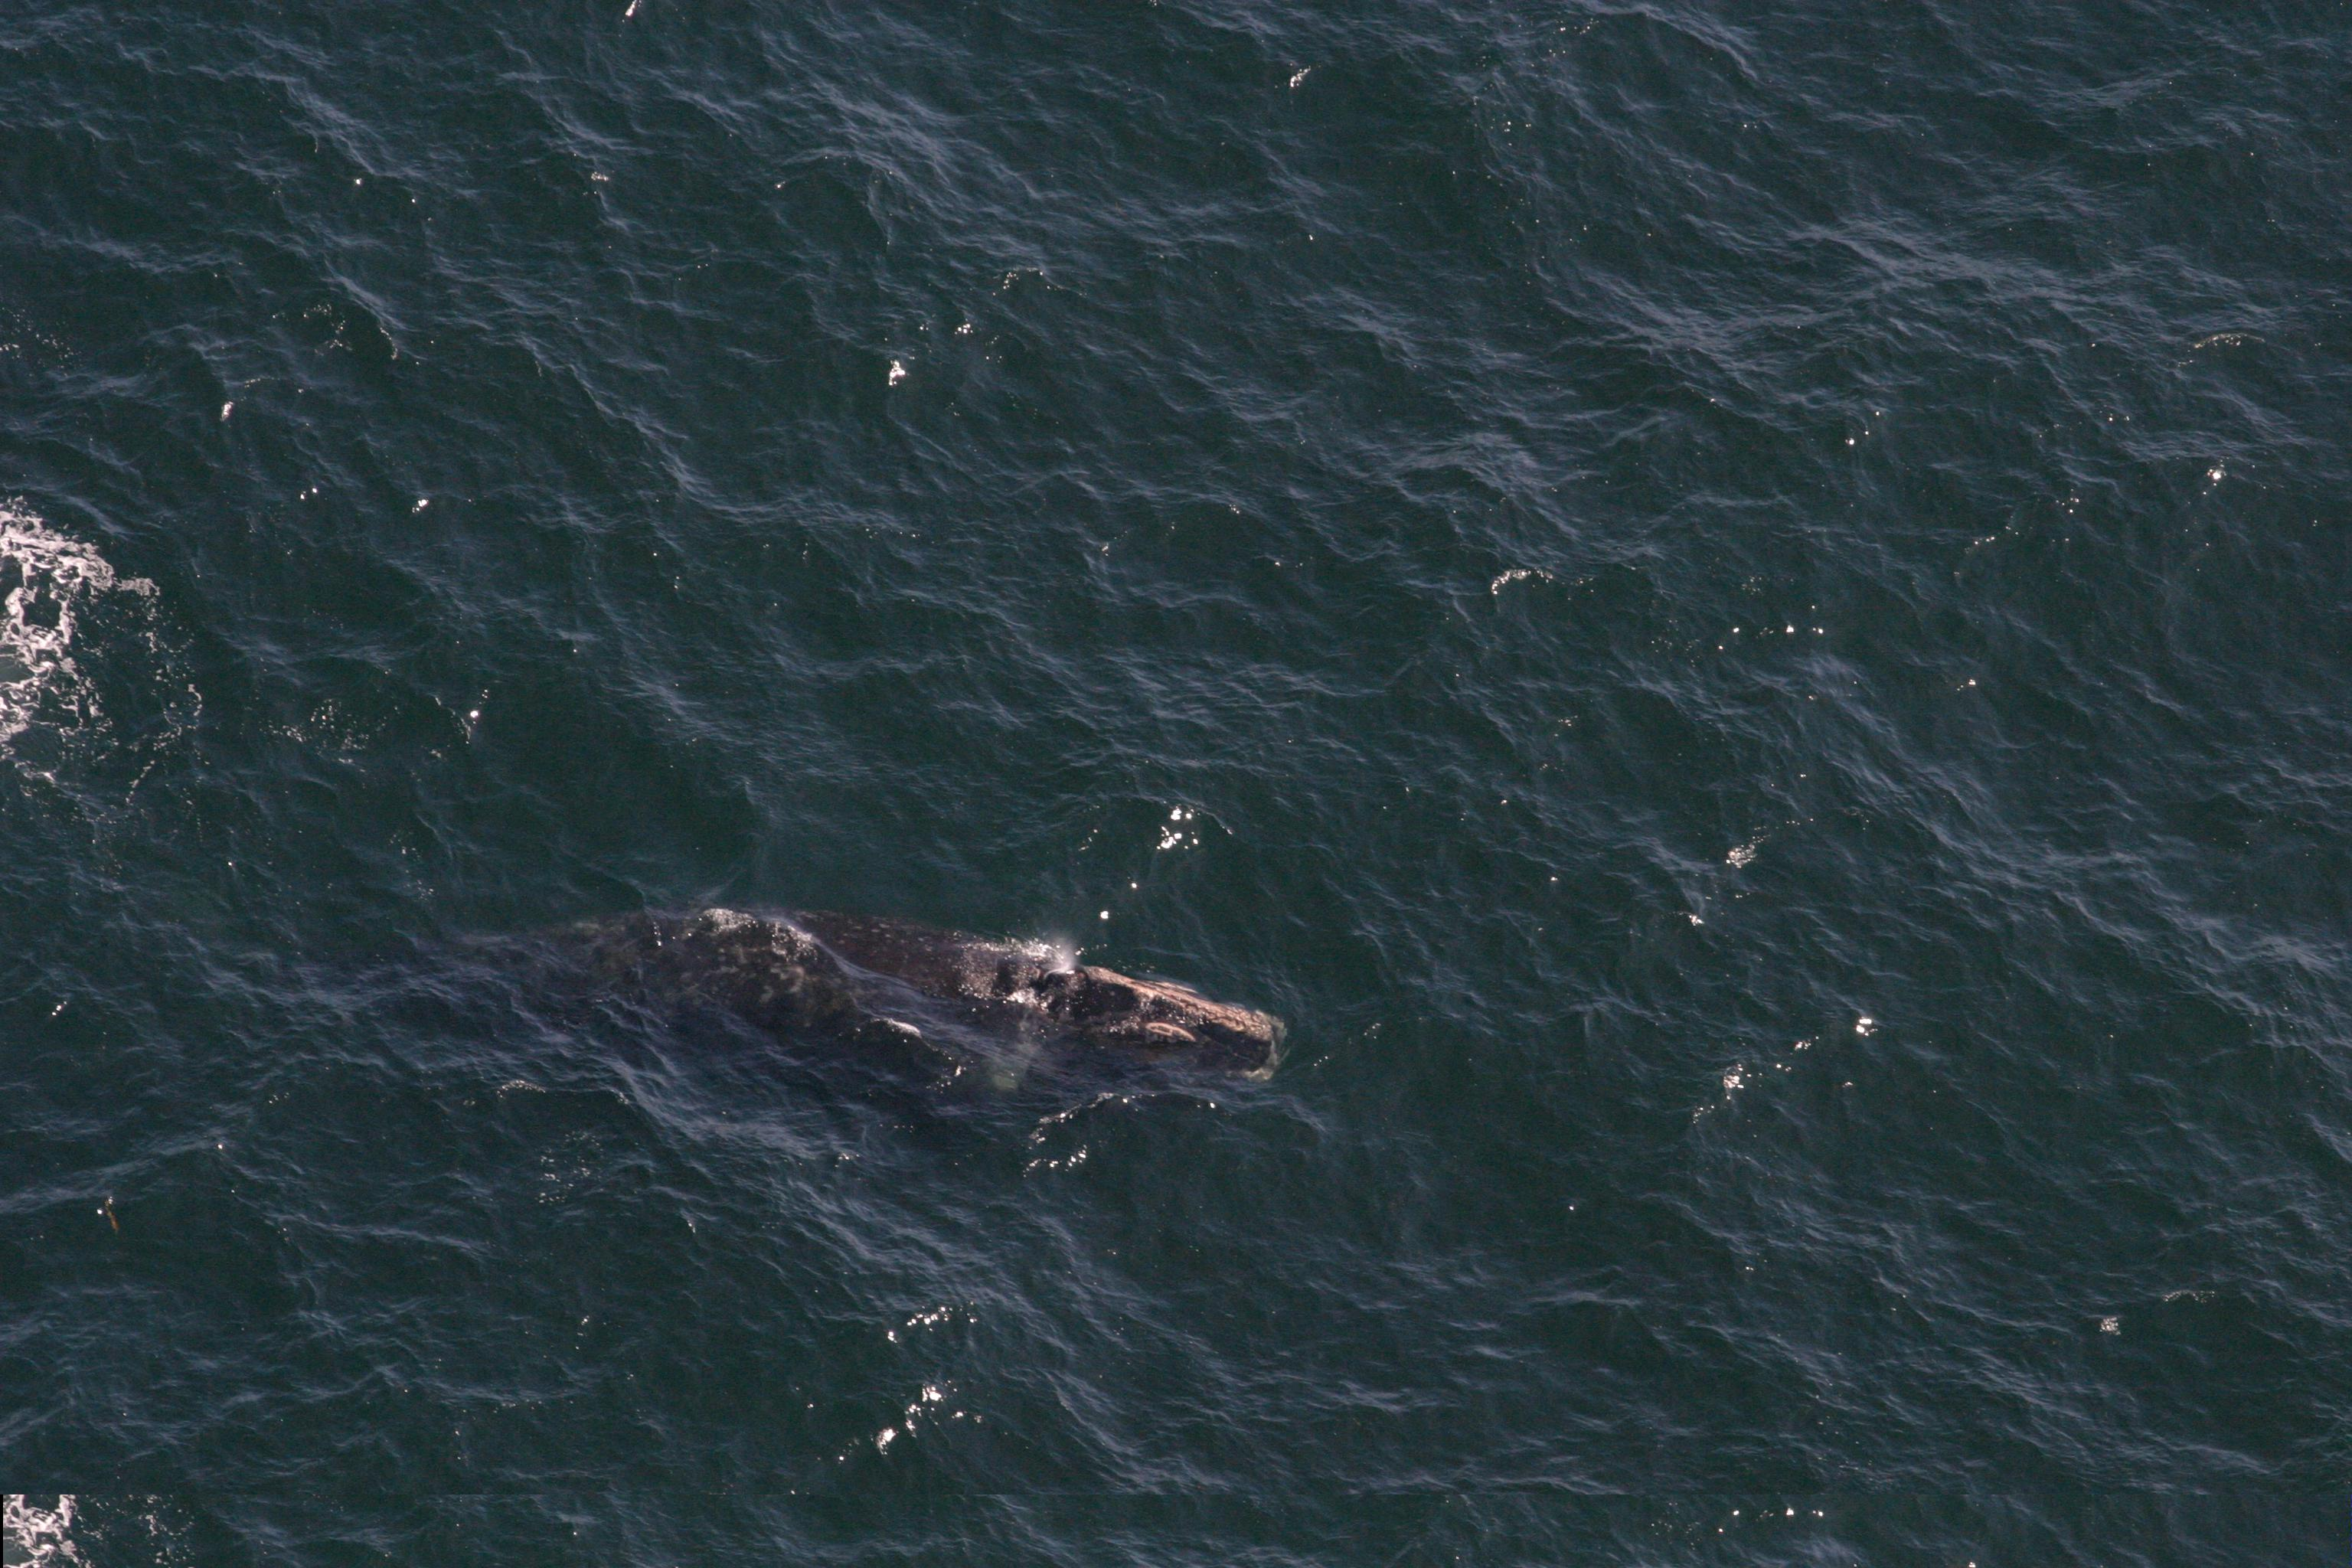
\includegraphics[width=\linewidth]{Images/w_7489}
	\caption{Example of whale from the dataset}
	\label{fig:whale-example}
\end{figure}

Another important thing to note about the dataset is the distribution of unique whales within the training data, an illustration of this can be seen in Figure \ref{fig:whale-frequency}. From this distribution it is notable that some whales are in a lot more images compared to some of the other whales. The results of the distribution can be seen in Table \ref{table:whale-distribution} where the minimum number of images for a whale is 1 and the maximum is 47 with an average of 10,47 and a standard deviation of 6,8.

\begin{table}
	\centering
	\caption{Unique distribution of whales in the dataset}
	\label{table:whale-distribution}
	\begin{tabularx}{\linewidth}{|l|l|}
		\hline
		Min & 1 \\ \hline
		Q1 & 5 \\ \hline
		Median & 9 \\ \hline
		Mean & 10,17 \\ \hline
		Q3 & 14 \\ \hline
		Max & 47 \\ \hline
		SD & 6,8 \\ \hline
	\end{tabularx}
\end{table}

\begin{figure}
	\centering
	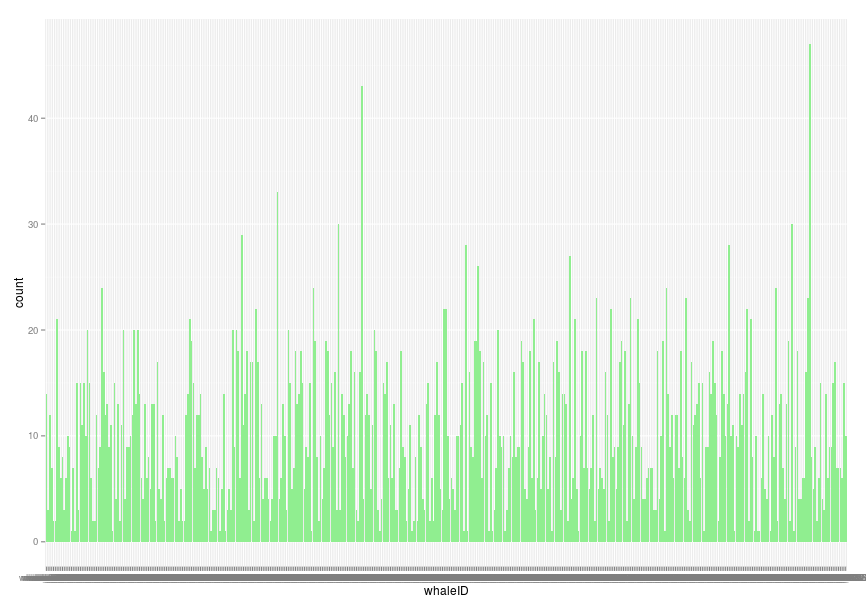
\includegraphics[width=\linewidth]{Images/FrequencyPlot}
	\caption{Frequency of unique whales in the training data}
	\label{fig:whale-frequency}
\end{figure}	

\section{Literature survive}
Before starting the project several areas was investigated to understand the North Atlantic Right Whale better and to see what other had done to perform classification on images, and what preprocessing techniques could be used.

\subsection{North Atlantic Right Whales}
Through the last decades the North Atlantic Right Whale have become an endangered whale species \cite{NOAA}. The North Atlantic Right Whale have been added to the list of animals under the protection of ESA\footnote{The Endangered Species Act} in 1931. The problem of this convention is that both Japan and the Soviet Union did not sign the agreement. Consequently, meaning that commercial whaling of the North Atlantic Right Whale to a large extend continued until 1949 where the whale species came under the protection of the International Convention for Regulation of Whaling. 
This convention deals with regulation of commercial whiling, but does not prohibit commercial whaling. 
This lead to an over-utilization of whaling in its primary habitat. The result of the commercial over-utilization meant that in 1970 the whale were determined to be in danger of extinction. 
Further, over the next decade, it has been added to both Endangered Species Convention Act, and designated the Marine Mammal Protection Act (MMPA) as Depleted.

In 2015 it have been estimated that there is fewer than 500 individual whales left. Nowadays, fishing of the whale is completely prohibited, but there are still a number of threats for the survival of the North Atlantic Right Whale.
These threats are:
\begin{itemize}
	\item Ship collisions 
	\item Entanglement of fishing gear
	\item Habitat Degradation 
	\item Contaminants
	\item Climate/Ecosystem changes
	\item Disturbance of whale-watching activities
	\item Noise from industrial activities
\end{itemize}
To counter these threats and recover the population of the North Atlantic Right Whale a recovery plan was established in 1991 \cite{NOAARecovery}. 
The goal of this plan is to downgrade the status of the whale species from endangered to threatened.
To accomplish this goal the recovery plan states seven major recommendations to:
\begin{enumerate}
	\item Reduce or eliminate injury or mortality caused by ship collision
	\item Reduce or eliminate injury and mortality caused by fisheries and fishing gear
	\item Protect habitats essential to the survival and recovery of the species
	\item Minimize effects of vessel disturbance
	\item Continue international ban on hunting and other directed take
	\item Monitor the population size and trends in abundance of the species
	\item Maximize efforts to free entangled or stranded right whales and acquire scientific information from dead specimens
\end{enumerate} 

This paper contributes to number 6, concerning monitoring size and trends.

\subsubsection{Monitoring the population}
The task of monitoring population consist of the following major tasks:
\begin{itemize}
\item \textit{General Monitoring of population.}
\item \textit{Monitoring of habitats.}
\item \textit{Emergency response.}
\end{itemize}

The protection of the whales species is regulated worldwide but Coordinated nationally, and responded to locally. This requires a lot of knowledge sharing in order the coordinate the effort. The problem here is that the different individual local institutions can make better decisions and reduce there effort by having the shared knowledge of all the individual institutions.
Further, as it is know only a few people has the skill needed to actually identify individual whales.

For this reason, the a Photo-identification database have been created. This database contains a set of images of each individual North Atlantic Right Whale. 
These images can then be used by the local institutions to compare what whales they have seen with the database, thereby ease the identification of a whale and make sure that each different institute talk about the same whale when sharing knowledge. Besides the images it contains a location/sighting history and a log.
The problem that still remains is the accurate identification of a whale. Even though it is possible to browse through the database and compare the observed with the entries in the database unique identification is both time consuming and inaccurate from the non experts.
Even if the identification have to go through the experts, it will so be time consuming that local institutions will have to wait long periods of time for an answer.
Since time is a critical factor in the protection of the whales this would cause big problems.

\subsubsection{How to recognize the whales}
It is a common technique to use image recognition to identity unique whales, many species has physical markings where it is possible to identity individual whales based on those markings. The North Atlantic Right Whale is no different. Figure \ref{fig:whale-collosity} shows the most important physical markings for the whales, it highlights some of the areas where unique characteristics can occur, while the white callosity in the middle is the most significant to look at \cite{neaq:whale-identity}. Besides the callosity other marks can be used to identify the whales:

\begin{itemize}
	\item Crenelations along the lower lip (also called lip “ridges”)
	\item Distinctive white patches on the belly and chin
	\item A dip or depression in the rostrum that can be seen in profile
	\item Erosion of the callosity in the front of the bonnet refereed to as “tooth decay”
	\item Flukes that curve upwards as the whale dives
	\item White blow holes
	\item White fluke tips
	\item Gray lines behind the blow holes
	\item Divots in their backs
	\item White scars from a host of causes (including past entanglements in fishing gear, ship strikes, attacks by killer whales or false killer whales, skin lesions, and other unknown causes)
\end{itemize}

Some of these identifying marks can be inherited from a whales parents, while other markings are acquired through the whales life, for instance scars \cite{neaq:whale-identity-markings}.

\begin{figure}
	\centering
	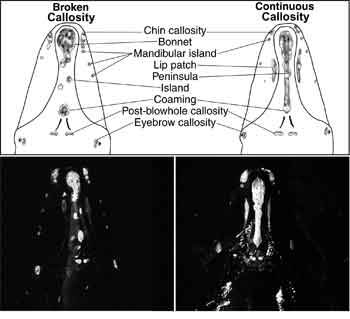
\includegraphics[width=\linewidth]{Images/callosity_comparison}
	\caption{Unique physical characteristics for North Atlantic Right Whales. Source: \cite{neaq:whale-identity}}
	\label{fig:whale-collosity}
\end{figure}

\subsection{Classification of images}
It was known beforehand that using Machine Learning algorithms could be used to classify images. What needed to be answered was which algorithms and techniques could be used for image recognition. 

The project is basically a facial recognition for whales, so research about how facial recognition systems work and what algorithms they use were done. Searching for articles, there are many implementations using different machine learning techniques, however some algorithms are more frequent than others. For instance the lecture from the CMU\footnote{Carnegie Mellon University} \cite{lit:nn1} explains how to use neural networks for facial recognition and argues that it is one of the best techniques to use. Likewise the article from \cite{lit:nn2} describes how a specific implementation of a neural network, called Convolutional Neural Network is working exceptionally good on recognizing and classifying images. 

Other algorithms which seem to have noteworthy results is the Random Forest, which are used in the following articles \cite{lit:rn1} and \cite{lit:rn2} both have good results and the Support Vector Machine algorithm is used in these articles \cite{lit:svm1} and \cite{lit:svm2} also solves the problem sufficient.

Many other articles mention these algorithms as some of the best for doing facial recognition, which leads to the assumption that they would probably work well for doing the image recognition needed to classify the individual whales.

%% Facial Recognition

% Neural Network
% - (1) http://web.archive.org/web/20030621155420/http://www-2.cs.cmu.edu/~tom/faces.html
% - (2) http://deeplearning.cs.cmu.edu/pdfs/Lawrence_et_al.pdf

% Random Forest 
% - (3) http://www.security.iitk.ac.in/contents/publications/mtech/VidyutGhosal.pdf
% - (4) https://kbsg.rwth-aachen.de/~schiffer/bib/icpr2008rff.pdf

% SVM
% - (5) http://cbcl.mit.edu/publications/ps/iccv2001.pdf
% - (6) http://papers.nips.cc/paper/1609-support-vector-machines-applied-to-face-recognition.pdf

\subsection{Preprocessing images}
\label{sec:litterature}
- How to filter out background

\section{Tools and Languages}
In this project several different languages and tools have been used. The following list contains a description of each of them. 

\begin{itemize}
	\item \textit{R} is an open source programming language used to write the main project. In R the following noteworthy packaged have been used
		\begin{itemize}
			\item \textit{cclust} is used for running the clustering.
			\item \textit{ggplot2} is used for creating the graphs
			\item \textit{EBImage} is used for image processing
		\end{itemize}
	\item \textit{H2O} is a open source data analysis tool written in Java with libraries to be used from Java, Python and R. H20 is created by 0xdata. H2O Have been used for running Random Forest and Neural Network Algorithm \cite{H2O}.
	\item \textit{ImageMagick} is used for handling image processing \cite{ImgMag}
	\item \textit{Java} is used for running some scripts for varies tasks
	\item \textit{Bash} is used for running some scripts for varies tasks
\end{itemize}


\section{Methodology}
\label{sec:methodology}
Describes which method has been used in the attempt to correctly classify North Atlantic Right Whales from images.

\subsection{Classification Algorithm}
Also known as \emph{Supervised Learning Algorithm}. Classification algorithms have one thing in common, which is that they require data input to be on a similar data structure.
The overall data structure for classifications is that it can contain 1..n observations which each has x amount of data points. For a model, the amount of data points for each observation has to be the same. An example as seen in Table \ref{tab:example data} shows how data could look.
If an observation is missing a value, it can be set to NA\footnote{Not Available} instead. It still has to be present in the structure.

\begin{table}
  \centering
  \caption{Example data}
  \label{tab:example data}
  \begin{tabularx}{\linewidth}{|l|X|X|X|X|} \hline
    obs. & x1 & x2 & x3 & x4 \\ \hline
    1    & 20 & 74 & 84 & 82 \\ \hline
    2    & 52 & 33 & 4  & 36 \\ \hline
    3    & 78 & 55 & 57 & 3  \\ \hline
    4    & 61 & 68 & 65 & 5  \\ \hline
  \end{tabularx}
\end{table}

\subsubsection{Decision Tree}
Decision tree is a classification algorithm. 
A decision tree is a binary tree structure where the path in each node is decided based on a split on a given input variable.
This variable split is configured to limit the amount of possible classes down each path. This is done by calculating the entropy (information gain) on each split on a given input variable/feature. This is then done for all input variables. A higher information gain means that a certain split separates different classes better.  
At the end of a path, a leaf contains the class to represent that exact path.
When prediction against a decision tree, that leaf is given as the returned prediction.

\subsubsection{Random Forest}
Random Forest is an algorithm which is based upon the decision trees and wisdom of the crowd.
Random Forest spawn multiple decision trees, the algorithm for splitting in the decisions tree in random forest does however differs from how it is done in normal decisions trees.
Random Forest use ``feature bagging'' at each node and then decide for the splitting feature on that subset rather than all the features. This ensures that decision trees is not identical, but offers variety.

\subsubsection{Neural Network}
Neural Networks is an algorithm as an attempt to mimic how the human brain works.
Neural Networks do however variate from how neurons and connections works in the brain as it contains a link from each node in layer x to each node in layer x + 1. As seen at Figure \ref{fig:neuralnetwork}, a neural network with only an input layer and an output layer is shown and the connections between the nodes. Each input node in the figure is connected to all the output nodes.

\begin{figure}
  \centering
  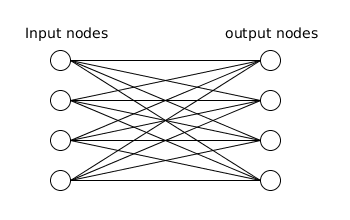
\includegraphics[width=0.7\linewidth]{Images/neuralnetwork}
  \caption{Neural Network with no hidden layers}
  \label{fig:neuralnetwork}
\end{figure}

\subsection{Clustering}
Is an \emph{Unsupervised Learning Algorithm} and was used for the preprocessing of the dataset. The specific implementation of the clustering used was K-Means. It splits the data into n clusters and uses euclidean distance to calculate which cluster to add new observations to. Every time new data is added, the center of the clusters are recalculated.

\subsection{Preprocessing tasks}
In the initial dataset there have been identified a number of inappropriateness which has to be ruled out before working with the data.
These inappropriateness are:
\begin{itemize}
\item Varying dimensions
\item Hugh dimensions
\item Too much noise in the dataset
%\item Positioning
%\item Rotation
\end{itemize}
These problems have been split into two different preprocessing tasks, Dimensional Reduction and Isolation of the whale.

\paragraph{Dimensional reduction}
As mentioned in Section \ref{sec:descr-of-data}, there are varying dimensionality in the dataset. Beside the varying dimensions, is the images too big to process. It is way too time consuming to process machine learning algorithms on images with approximating 3000x2000 pixels in RGB, since the number of dimensions then would be:
\begin{equation}
Dimensions = 3 \times 3000 \times 2000=18.000.000
\end{equation} 
Further is it not given that more dimensions will provide a better result.
Therefore, one preprocessing task is to down scale the images.
The down scale used in this project will be around 45x30 pixels, giving the vectors 4050 dimensions.
Further dimensional reduction is to use gray scale instead of RGB, or simply use binary (\emph{black/white}) generated with a threshold.

\paragraph{Isolating whale}
The problem with reducing the dimensions through scaling, is that the whale is a relatively small part of the images. Figure \ref{fig:scale} shows one of the original images from the dataset and the same image down scaled to 45x30 pixels. As seen from the figure is the whale nearly non existing in the new scale. The whale on the down scaled image is sanding of two pixels.  
Further as the water is noise without information about the whale using computational time on processing it is simply a waste.
\begin{figure}
	\centering
	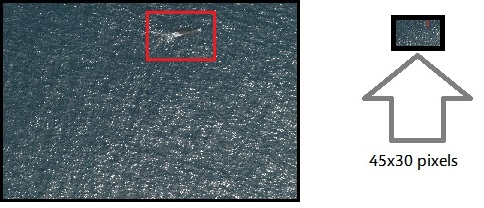
\includegraphics[width=\linewidth]{Images/scale}
	\caption{One picture from the data marked with a red square around the whale, and on the left the same image, down scaled to 45x30 pixels}
\label{fig:scale}
\end{figure}

In order to get more information about the whale it have been decided to develop a system to crop the images to the whale, thereby allowing more information about the actual whale being present in the down scaled images.

\subparagraph{General Principle}
The general principle behind the cropping is  assumption that there is a true difference between what is whale and what is water. Further, do we assume that water pixels, even though there are differences, look more alike than whale pixels and water pixels.
Because of it is assumed that a clustering algorithm could separate water from whale.
In order to lower error rate of this separation there are a number of major parameters:
\begin{itemize}
\item \textit{Smoothing.} By smoothing the image before clustering the pixels, the individual values for the different pixels are equalized based on the neighboring pixels. By doing so, water pixels will look more alike as will individual whale pixels.
\item \textit{Scale.} This will presumably have the same effect as smoothing of the image. But this will also increase performance since it will reduce the number of dimensions.  
\item \textit{Number of clusters.} In order to separate water from whale only two clusters are needed. But this might have some problems if there are more than just water and whale on the image. For instance, does water splash pixels distinguish themselves from both water and whale and by having  only two clusters there would be no control of which cluster these will end up in. They might in fact get one of the clusters for themselves, leaving water and whale in one cluster.
\item \textit{Distance algorithm.} Which algorithm used to determine the distance between pixels might affect of well the separation is done. As mentioned in Section \ref{sec:litterature}, is it suggested to use an euclidean distance
\item \textit{Features.} Using the RGB or gray scale values might not be the best way of separating the data. Another way could be to use redness (how red a pixel is compared to green and blue) since the whale is more red than the water. Further could a value for the distance from average pixel value, for each pixel be used. This might be performing well since most of the image is water therefore the feature would approximately describe one pixels distance from what is water causing all water pixels to be approximately zero and other pixels to be not zero.
\end{itemize}


\section{Results and Evaluation}
This section explains the results of the project in \ref{subsec:results} and evaluate on the results in \ref{subsec:evaluation}.

\subsection{Results}
\label{subsec:results}
This section contains results for both the preprocessing and the two classification algorithms and their performance.

\subsubsection{Preprocessing}
The preprocessing was done in the following steps.
Initially the images was downscaled to 100 pixels width.
Images was normalized using Z-Score normalization resulting in the right image of Figure \ref{fig:step1}. By normalizing the images the contrasts becomes greater and this will ease the separation.
In the next step, the image is smoothed with a Gaussian smoothing algorithm with a sigma level of 2. This equalizes the values of the individual pixels a bit and thereby make neighboring pixel more alike.
When these steps are done, two features are extracted from each pixel.
These features are the redness and a gray scale value.
The features are then used for the K-Means clustering algorithm.
The clusters are constructed using Euclidean distances. Further is the algorithm constructed to build 4 different clusters.
The reason for using four clusters, is that it is expected that water, water splashes, whale and 'garbage' will be in their own separate cluster.

When the clusters are created the next step is to identify which cluster(s) the whale have been added to.
This is done by finding the cluster which has the highest rate of redness within it. This works for most of the images but not all. In some images the contrast between whale and water is not high enough or the light when the image was taken makes the water splashes red. When this happens, the correct cluster is chosen by calculating the center of gravity in the image. After the center of gravity is calculated the cluster in which it is placed is picked, if the size of that cluster is between 5 \% and 20 \% of the total. This picks the correct cluster with an accuracy of around 50 \%.
When it fail to find a cluster, a cluster matching the size for 10-15 \% of the total image is taken \footnote{Note that the last approach might choose a wrong cluster, and cannot be validated, which is why the two other approaches are preferred}. 

When one or more cluster is chosen, everything not in that cluster is filtered out from the original smoothed image as seen in Figure \ref{fig:step3} right. The whole process is then repeated once more in order to filter out some few water pixels which was gathered in the whale cluster.
After the second round a minimum bounding box is calculated around the whale cluster, and the image is then cropped.

\begin{figure}
\centering
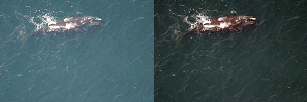
\includegraphics{Images/preprocess1}
\end{figure}

\subsubsection{Random Forest}
The Results for Random Forest is split into two sections. As there has been conducted classification for both data which was just resized and data which has been additionally preprocessed before resizing.

\paragraph{The Resized Data}
\label{par:rf-resized}
Shown in Figure \ref{fig:random-forest-resized}, an averaged result of 3 fold cross validation. The graph is shown with a one-tailed 95\% confident interval with a degree of freedom on 3. The criteria of interest is the potential worst performance of the model. Which is the upper line of the embedded error bar on the graph at each point. The cutoff line defines the performance at random selection, which is 1 / 447. 

Each validation point for the chart correspond to the number of trees in the forest, plus 1 additional tree. So for validation point ``5'', the model has 6 trees.

The performance of the test set for Figure \ref{fig:random-forest-resized} do for each validation point have a \emph{significant better performance} than choosing random selection.

The training set does significant better than the test set, but just states that the model is overfitted and should be trained against more observations to introduce more variety.

\begin{figure*}
  \centering
    \begin{subfigure}{.5\linewidth}
      \centering
      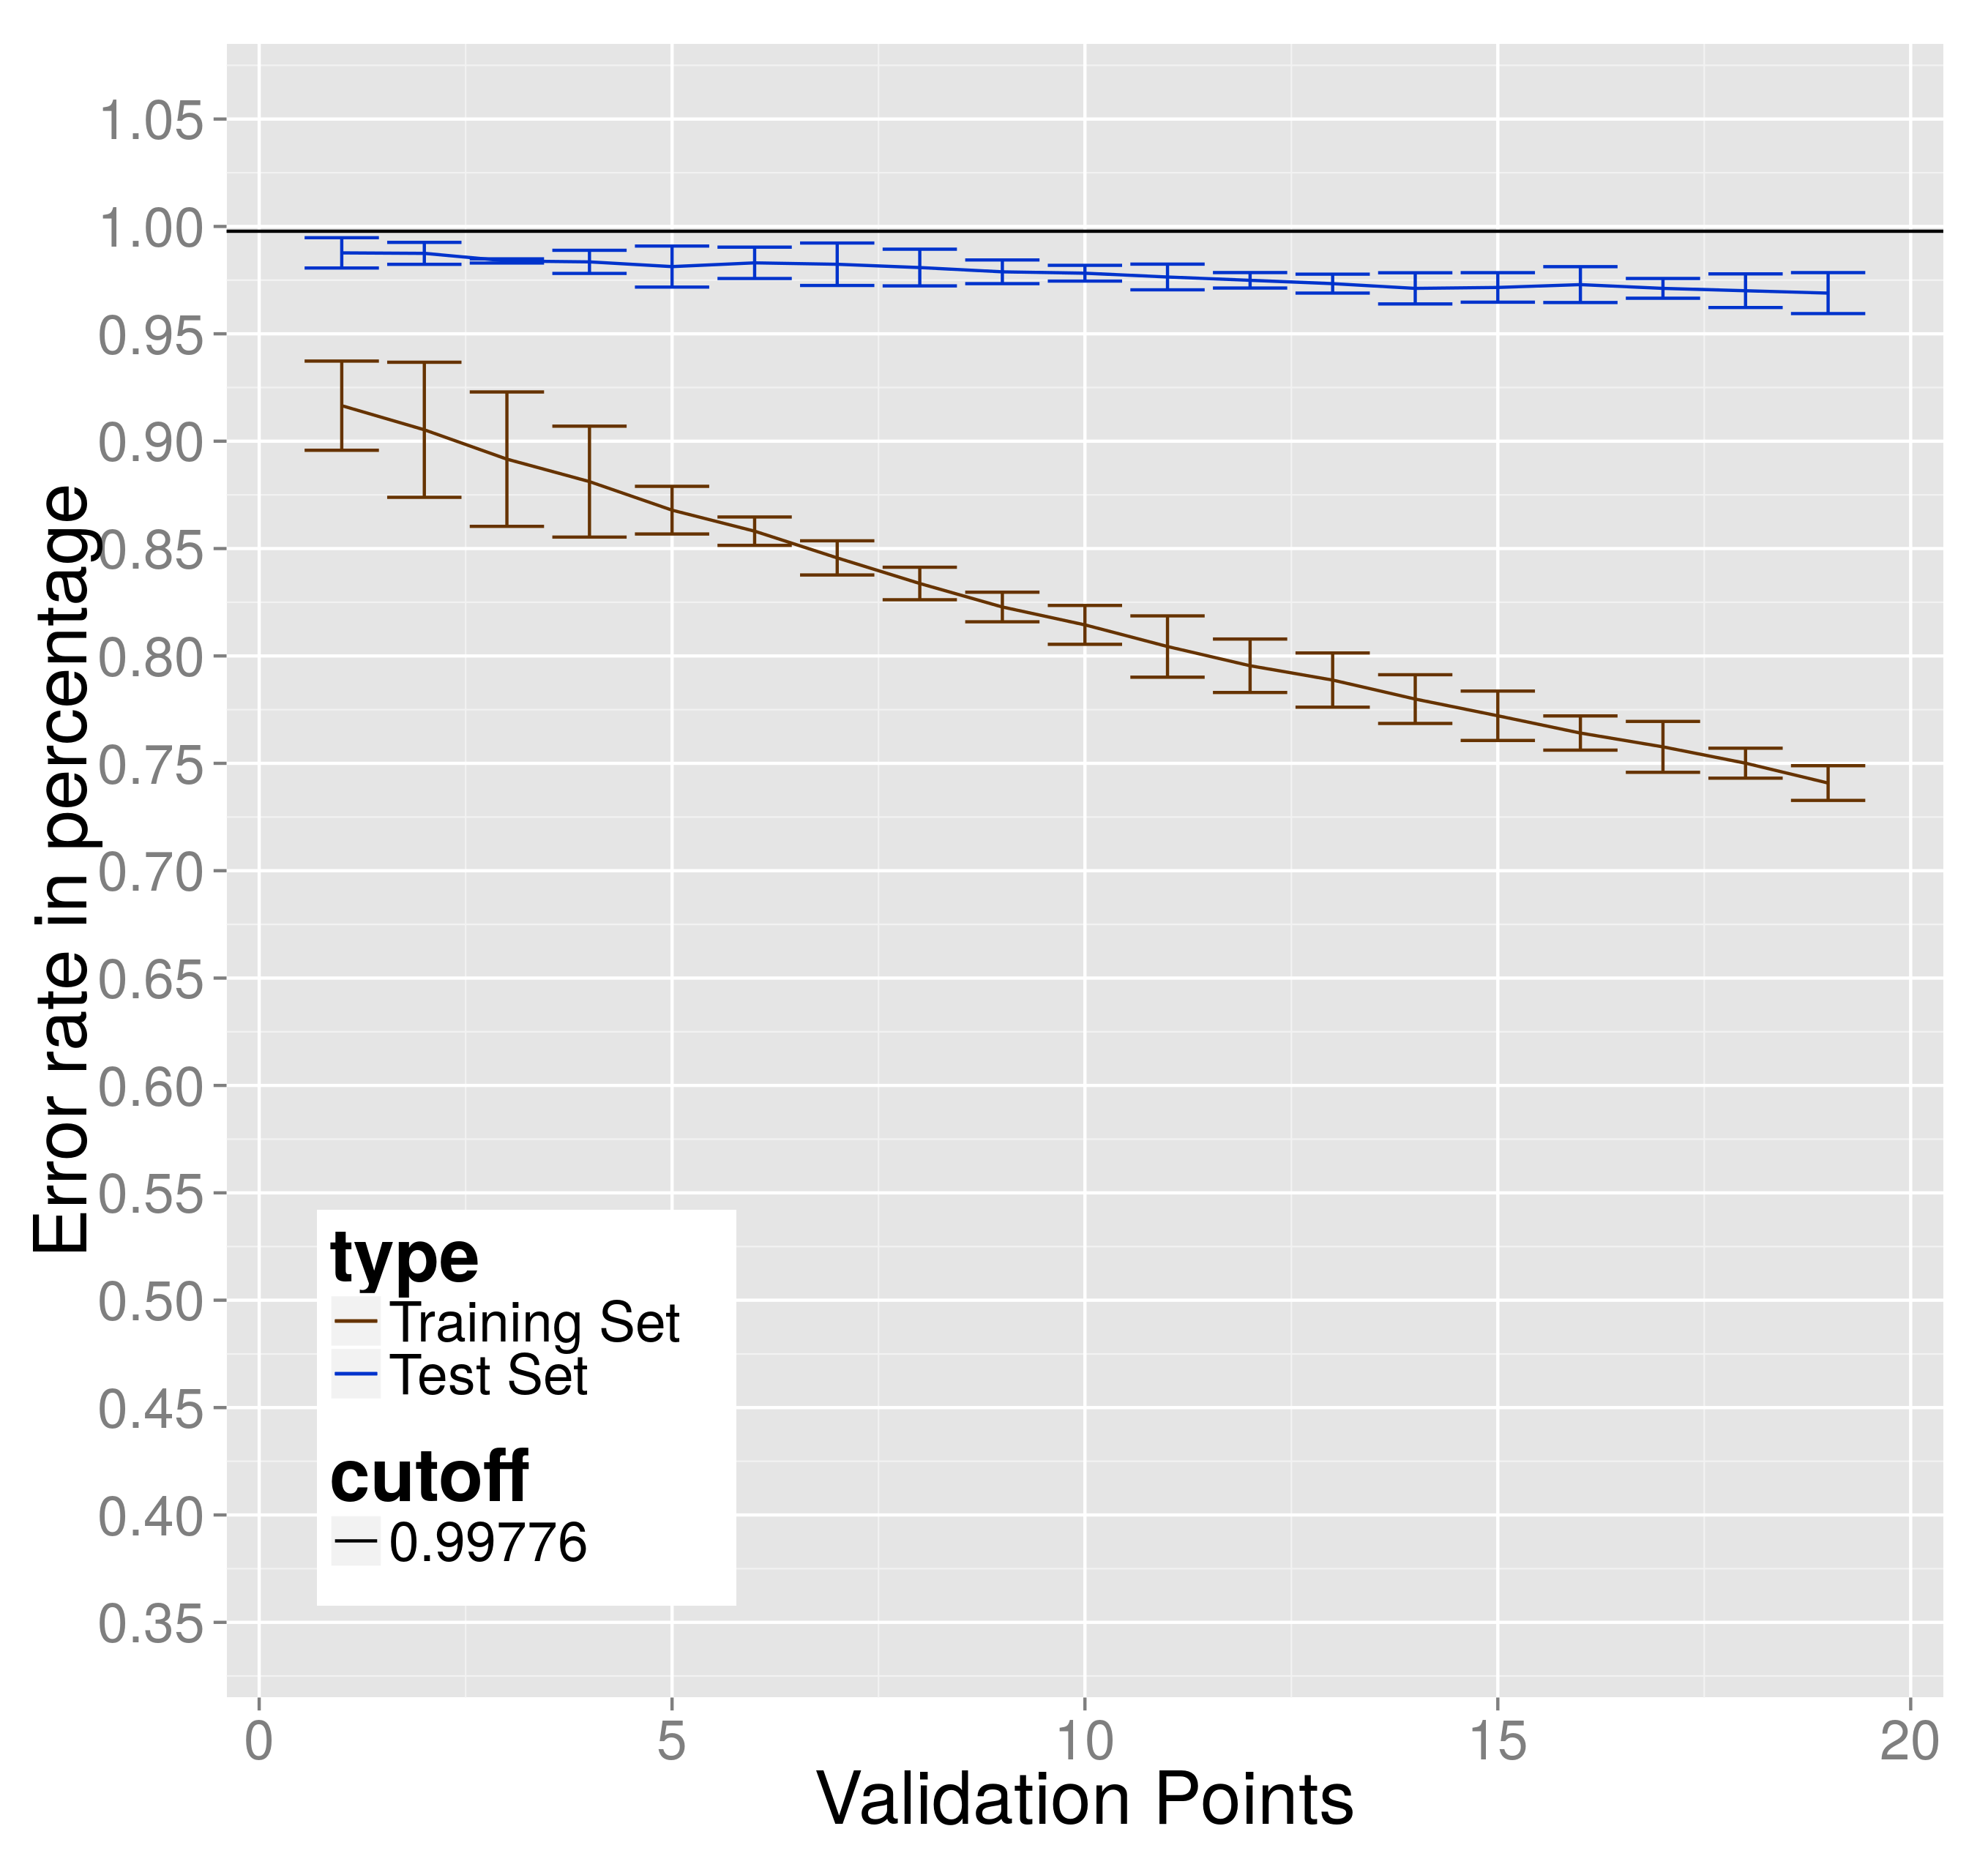
\includegraphics[width=0.95\linewidth]{Images/DRFraw}
      \caption{Without preprocessing}
      \label{fig:random-forest-resized}
    \end{subfigure}%
    \begin{subfigure}{.5\linewidth}
      \centering
      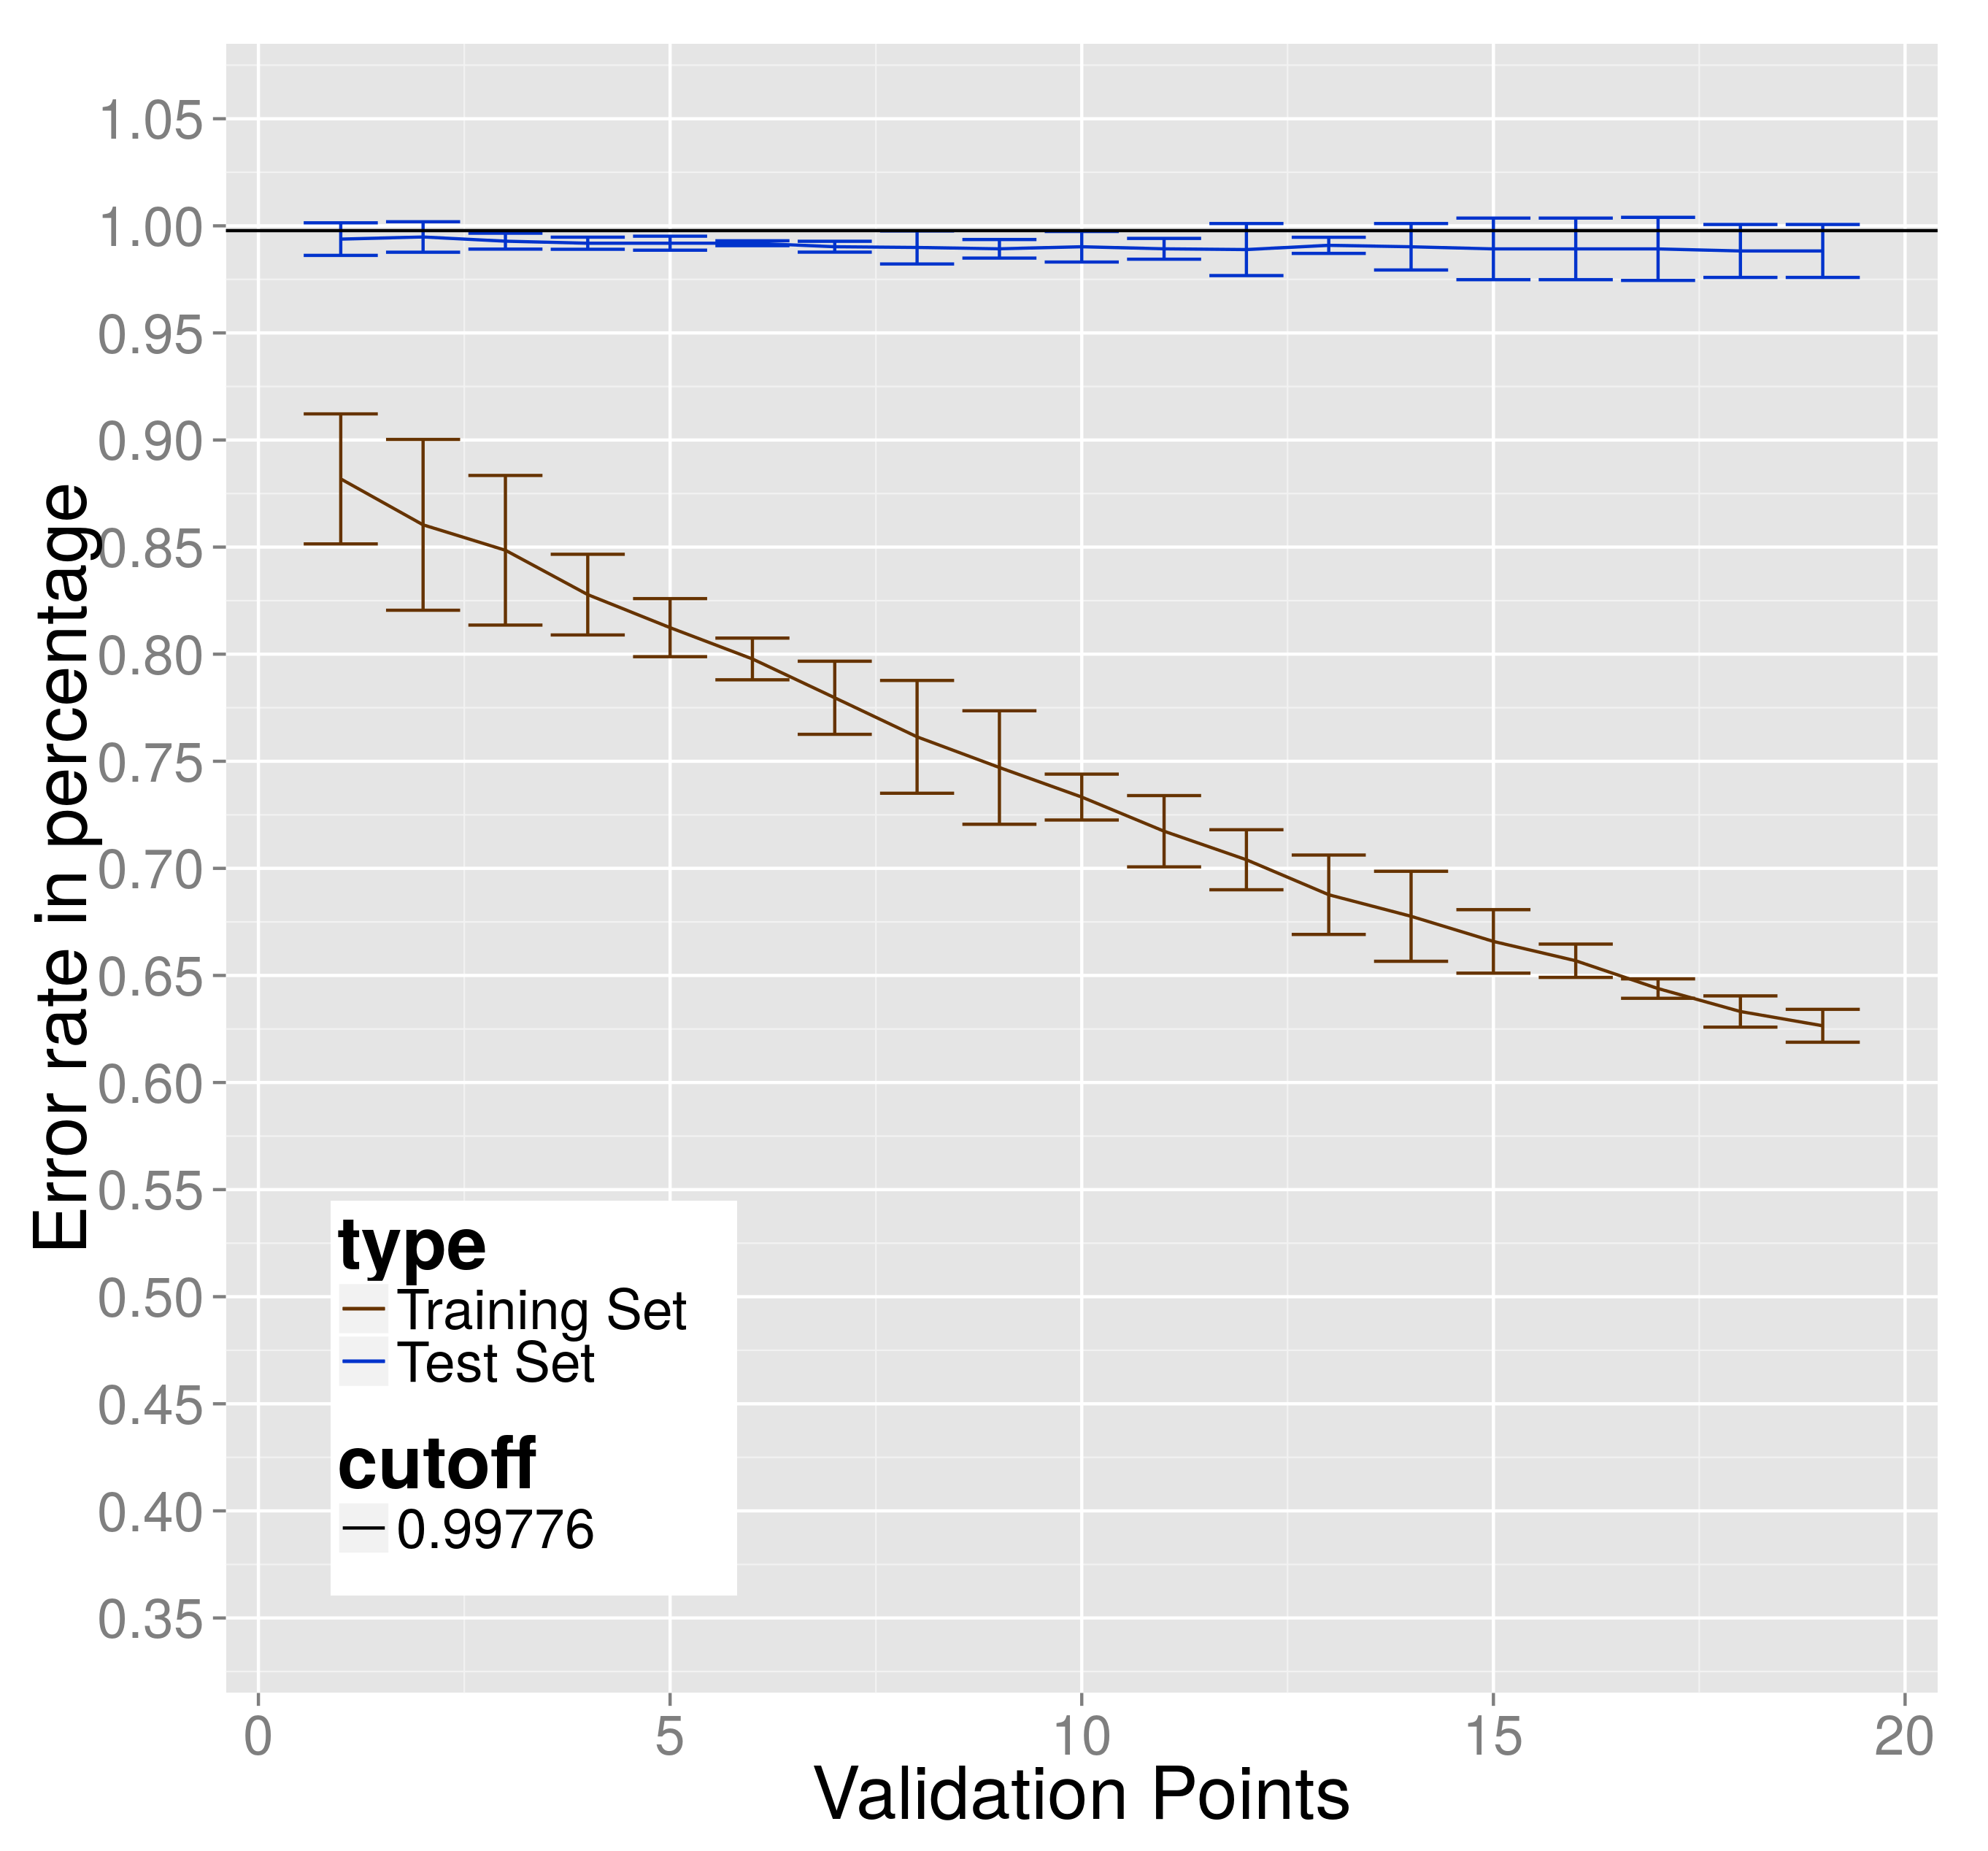
\includegraphics[width=0.95\linewidth]{Images/DRFpreprocessed}
      \caption{With preprocessing}
      \label{fig:random-forest-preprocessed}
    \end{subfigure}
  \caption{The results for Random Forest}
  \label{fig:random-forest}
\end{figure*}

\paragraph{The Preprocessed Data}
Shown in Figure \ref{fig:random-forest-preprocessed} follow the same conditions with 3 fold cross validation, one-tailed 95\% confident interval with degree of freedom on 3, as seen at \ref{par:rf-resized}.

The only different is the data input which uses the preprocessed data instead.
The test set \emph{do not} have a significant better performance than random selection, but do have some sweet spots at some amount of trees which seems better, but might as well be due to the limited amount of folds.

The training set shows the same issues as the only resized images shown in Figure \ref{fig:random-forest-resized}, also explained in \ref{par:rf-resized}.

\subsubsection{Neural Network}
\label{subsubsec:neuralnetwork}
This section contains the results from the neural network model using both the resized and the preprocessed datasets.

\paragraph{The Resized Data}
in Figure \ref{fig:nn-resized} shows two non-static lines and a static cutoff line.
The static cutoff line represent random selection for a correct classification, where as the two other lines show the test and training sets performance against the model at given validation points. Additionally a one-tailed 95\% confident interval at 3 degrees of freedom is shown as the error bar at each validation point for both lines.

The test set \emph{do not} have a significant better performance than random selection.

The training set do have a \emph{significant better performance} against the model compared to the test set, which shows overfitting also mentioned in \ref{par:rf-resized}

\begin{figure*}
  \centering
    \begin{subfigure}{.5\linewidth}
      \centering
      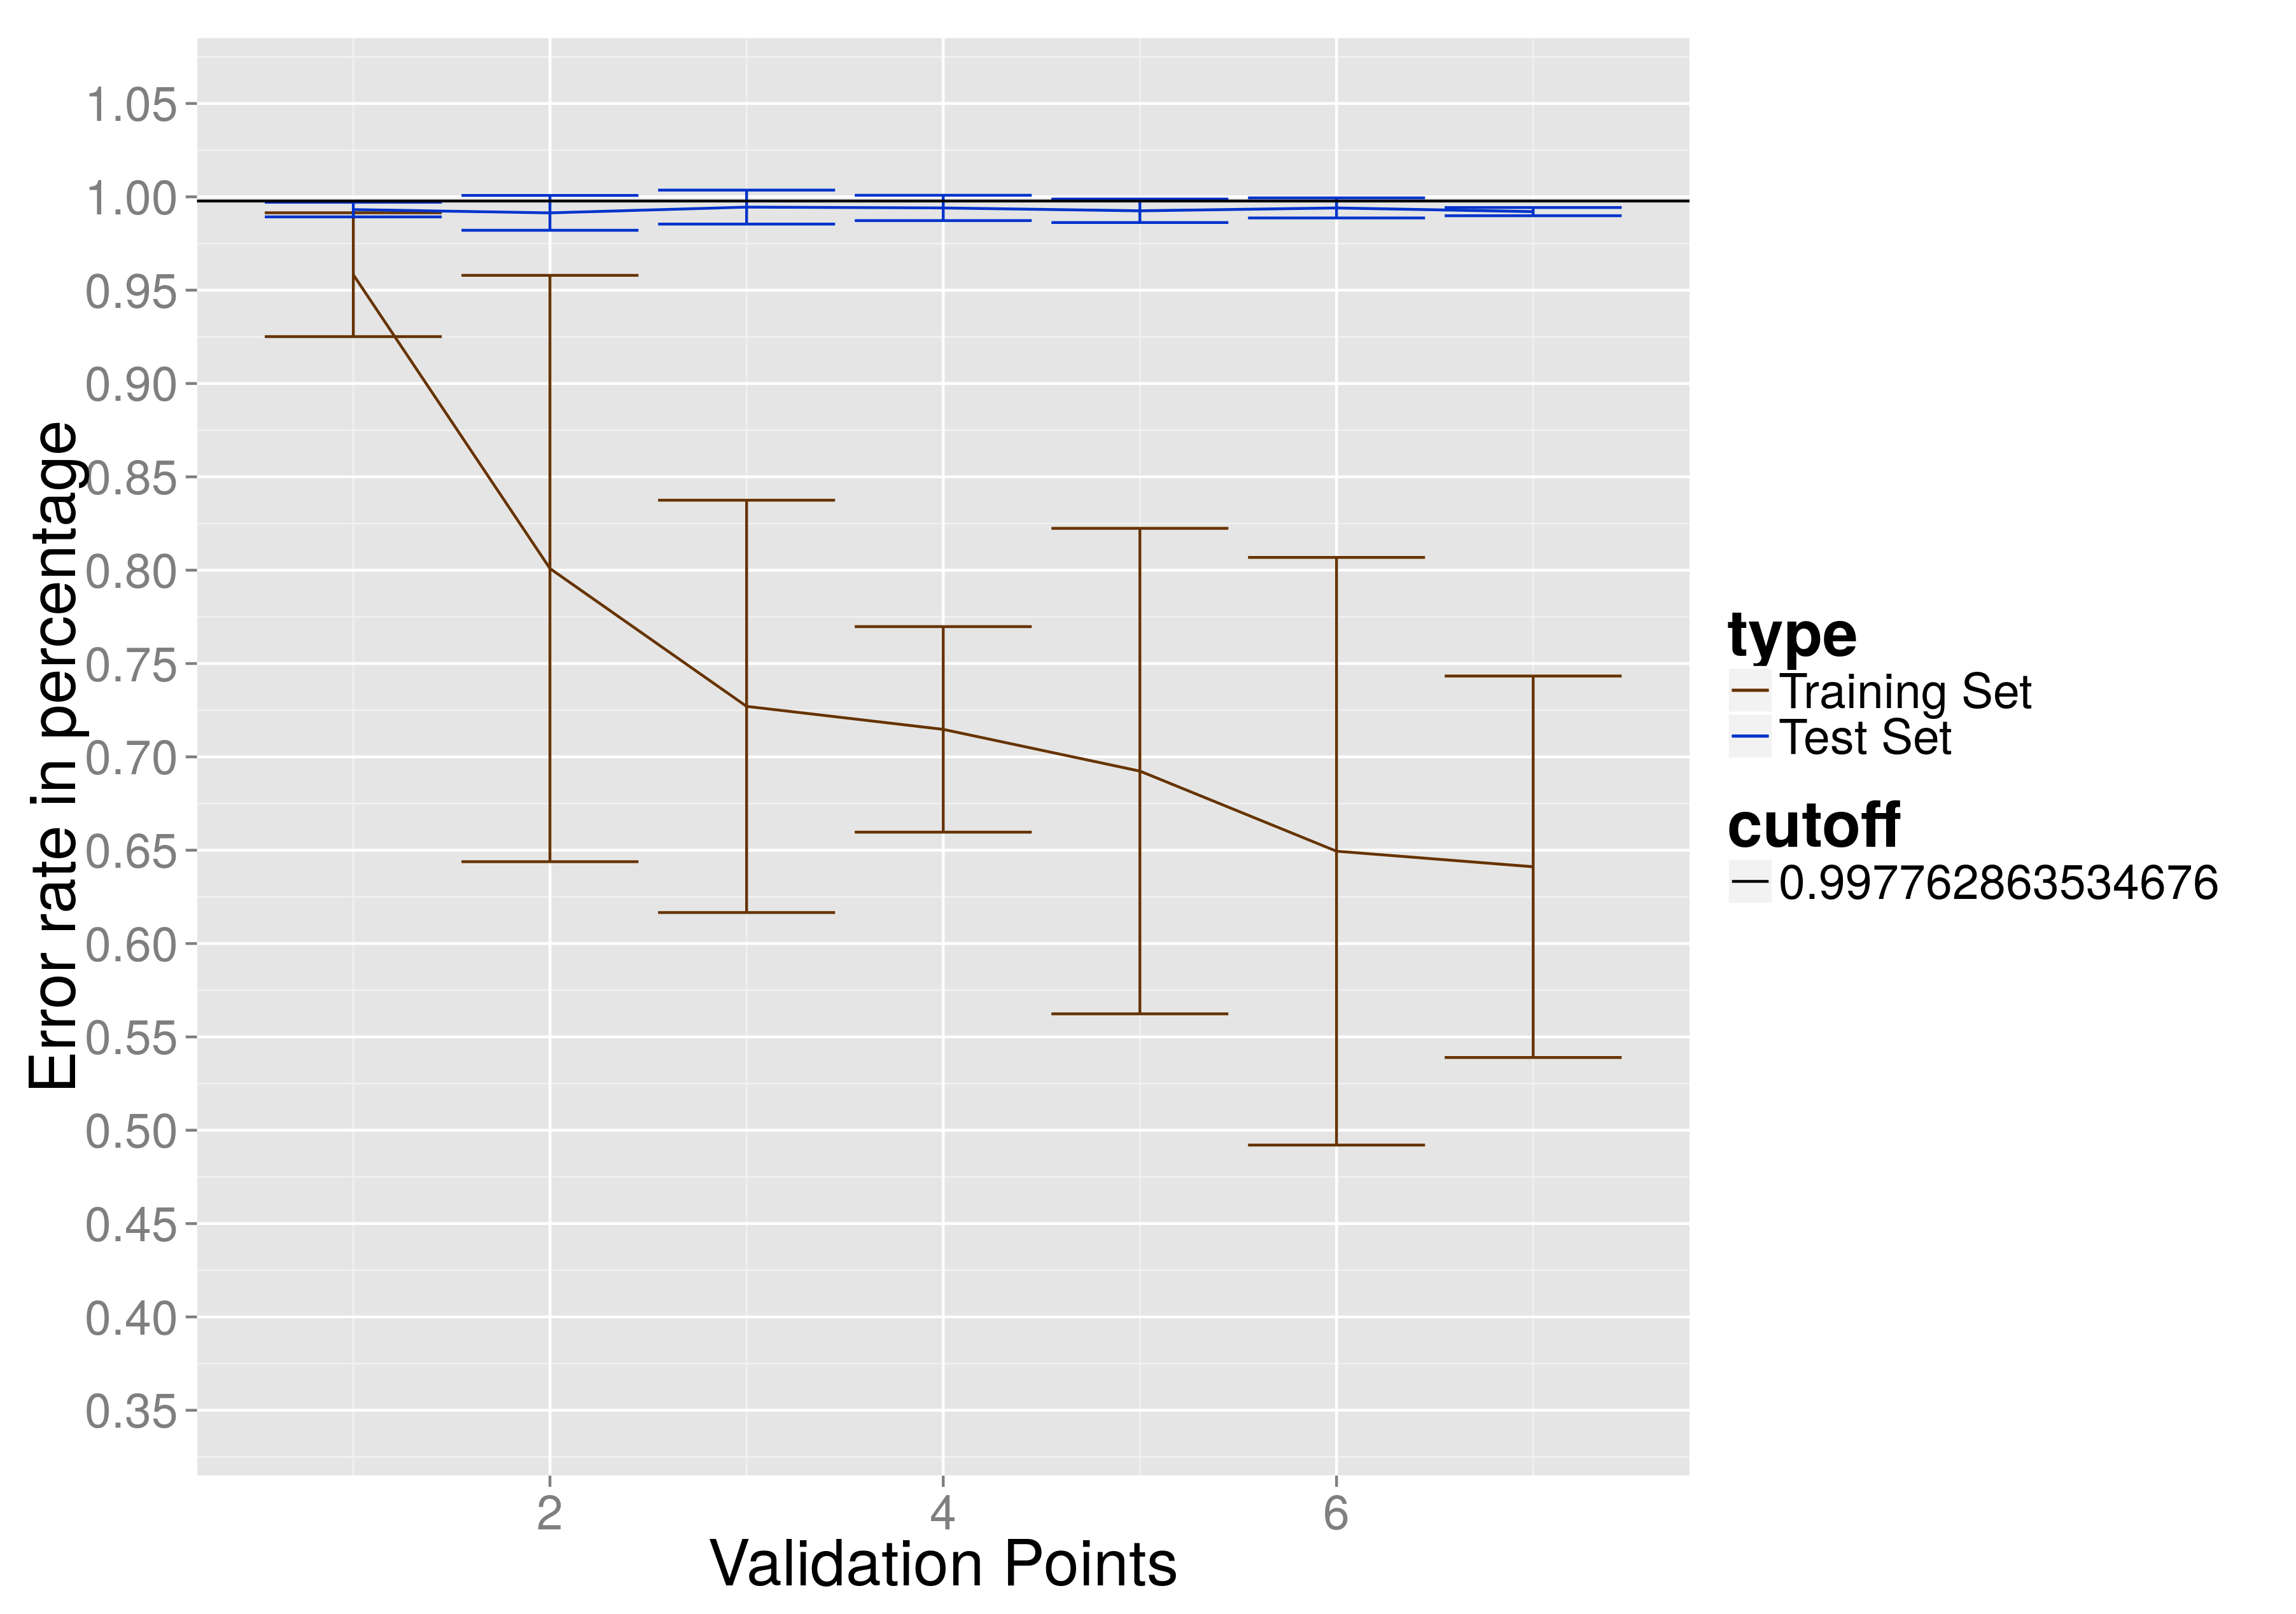
\includegraphics[width=0.95\linewidth]{Images/DNNraw}
      \caption{Without preprocessing}
      \label{fig:nn-resized}
    \end{subfigure}%
    \begin{subfigure}{.5\linewidth}
      \centering
      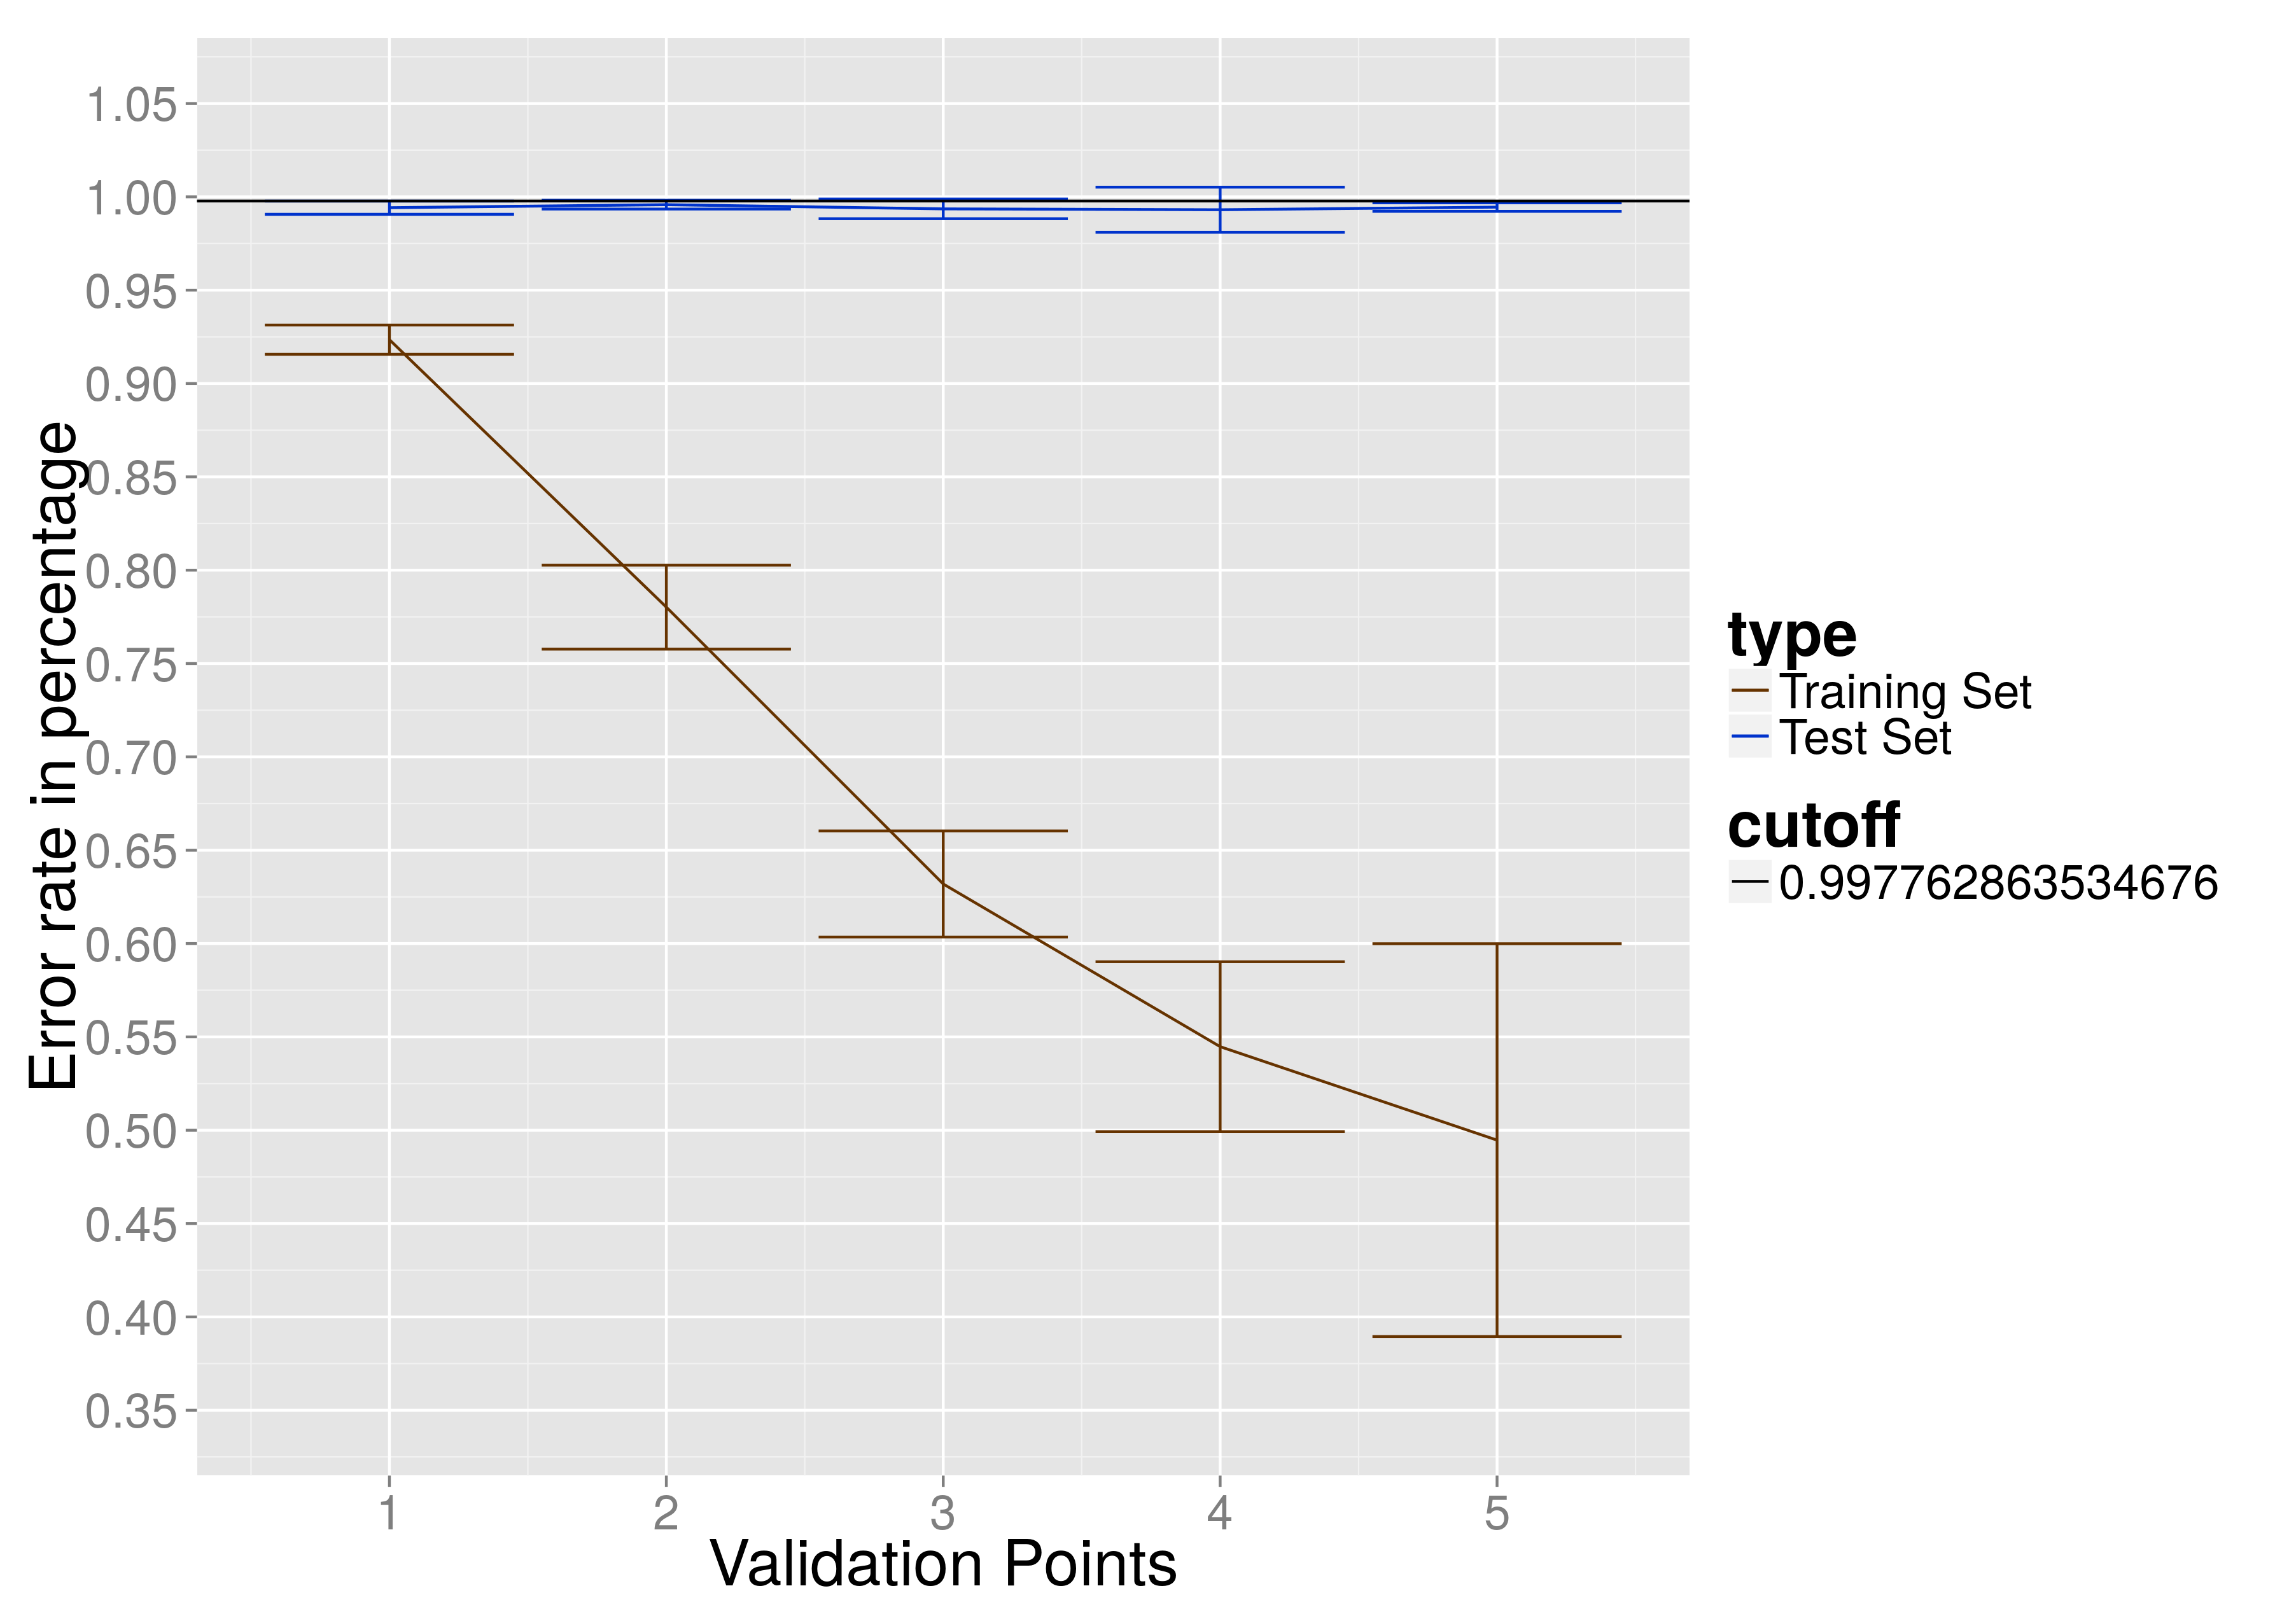
\includegraphics[width=0.95\linewidth]{Images/DNNpreprocessed}
      \caption{With preprocessing}
      \label{fig:nn-preprocessed}
    \end{subfigure}
  \caption{The results for Neural Network}
  \label{fig:neural-network}
\end{figure*}

\paragraph{The Preprocessed Data}
in Figure \ref{fig:nn-preprocessed} contains the same graph scheme as explained in previous paragraph in \ref{subsubsec:neuralnetwork}. 

The test set \emph{do not} have a significant better performance than random selection.

The training set do have a \emph{significant better performance} against the model compared to the test set.

\subsubsection{Result Conclusion}
The results for the four different experiments shows that only Random Forest on the resized data stands out as an \emph{significant better performance} compared to random selection.

\label{subsec:evaluation}

\section{Limitations}
After the poor accuracy of the results, ideas on how to drastically increase them were realized. Tweaking the settings of the algorithms would probably increase the accuracy of the results, but that would be no where enough to get what was desired. 

Therefore it was clear that the preprocessing had to be improved. Having enough computational power to use the images with larger dimensions could increase the accuracy, because the low dimensions has the risk of removing some important markings of the whale. Another approach could be to further crop the images to only contain the head/face of the whale allowing more information to be in smaller images.

Rotating the whales so they all face in the same direction could increase the results too, as the algorithms are unable to comprehend the relation between pixels, because they just compare the values relative to each other. So making sure all the whales are placed and look similar on all images should yield a better result. It would be required for all whales to be in the exact same position in all the images.

Since the algorithms do not comprehend the correlation between the pixels, an alternative solution would be to not use the pixels as features, but instead extract features which describes all the unique markings for the whales, this would make it easier to train the model to only look at those features in the image instead of looking at all the pixels.

The amount of data in the dataset is relatively small, with ~4500 entries, increase the size could provide better results, as some algorithms require large datasets to be trained correctly. It would also be better to have more samples for each whale, as only 10 images in average is not necessarily enough if the image is of poor quality in relation to extracting relevant features.

Some of the images contain whales which are unable to be identified, even by trained researched. Finding a way to rid those entries from the dataset could help train a better model, and as such increase the probability of getting a more accurate model.

\section{Conclusion}

The results have shown that Random Forest algorithm on non-preprocessed images gives the best results, with an accuracy of ~4 \% correctly classified images. This result have been computed with a 99.7 \% confidence of performing better than Random selection. This however, is the only result computed where the confidence is high enough to say that the performance is significant better.
The same algorithm on the preprocessed images gave a result of ~2 \% correctly classified images with a confidence of 91.5 \%.

For the neural network the performance was shown to be as bad as random selection, both with and without preprocessing with a confidence of 89 \% for original resized images and 78.5 \% for the preprocessed images.

The reason the used preprocessing gives a worse performance might be due to the fact that there are some other correlation between images. For instance the same whale might be photographed in the same geographical area and even with the same lighting conditions, giving the algorithm a "wrong" correlation between the data entries, which are minimized when the images is cropped.
Other reasons for the poor performance is due to the limitation stated in Section \ref{sec:limitations}.
To summaries these reasons are:
\begin{enumerate}
\item Size of images 
\item Further cropping
\item Position and angle of whale
\item Extraction of features
\item Bigger dataset
\item Pruning of data set
\end{enumerate}
These 6 steps of improvement are critical if better results are to be obtained with the given algorithms. 

%\subsection{Alternative Hypotheses}


%\bibliographystyle{plainnat}
\bibliographystyle{apalike}
\bibliography{references}

\appendix



\end{document}

